%%%%%%%%%%%%%%%%%%%%%%%%%%%%%%%%%%%%%%%%%
% Stylish Article
% LaTeX Template
% Version 2.2 (2020-10-22)
%
% This template has been downloaded from:
% http://www.LaTeXTemplates.com
%
% Original author:
% Mathias Legrand (legrand.mathias@gmail.com)
% With extensive modifications by:
% Vel (vel@latextemplates.com)
%
% License:
% CC BY-NC-SA 3.0 (http://creativecommons.org/licenses/by-nc-sa/3.0/)
%
%%%%%%%%%%%%%%%%%%%%%%%%%%%%%%%%%%%%%%%%%

%----------------------------------------------------------------------------------------
%	PACKAGES AND OTHER DOCUMENT CONFIGURATIONS
%----------------------------------------------------------------------------------------

\documentclass[fleqn,10pt]{SelfArx} % Document font size and equations flushed left

\usepackage[english]{babel} % Specify a different language here - english by default

\usepackage{listings}

%----------------------------------------------------------------------------------------
%	COLUMNS
%----------------------------------------------------------------------------------------

\setlength{\columnsep}{0.55cm} % Distance between the two columns of text
\setlength{\fboxrule}{0.75pt} % Width of the border around the abstract

%----------------------------------------------------------------------------------------
%	COLORS
%----------------------------------------------------------------------------------------

\definecolor{color1}{RGB}{0,0,90} % Color of the article title and sections
\definecolor{color2}{RGB}{0,20,20} % Color of the boxes behind the abstract and headings

%----------------------------------------------------------------------------------------
%	HYPERLINKS
%----------------------------------------------------------------------------------------

\usepackage{hyperref} % Required for hyperlinks

\hypersetup{
	hidelinks,
	colorlinks,
	breaklinks=true,
	urlcolor=color2,
	citecolor=color1,
	linkcolor=color1,
	bookmarksopen=false,
	pdftitle={Title},
	pdfauthor={Author},
}

%----------------------------------------------------------------------------------------
%	ARTICLE INFORMATION
%----------------------------------------------------------------------------------------

\JournalInfo{Not published} % Journal information
\Archive{} % Additional notes (e.g. copyright, DOI, review/research article)

\PaperTitle{Monte Carlo Methods and Hardware Acceleration} % Article title

\Authors{Johannes Gäßler\textsuperscript{1}*} % Authors
\affiliation{\textsuperscript{1}\textit{Department of Physics, Karlsruhe Institute of Technology, Karlsruhe, Germany}} % Author affiliation
\affiliation{*\textbf{Corresponding author}: johannes.gaessler@student.kit.edu} % Corresponding author

\Keywords{} % Keywords - if you don't want any simply remove all the text between the curly brackets
\newcommand{\keywordname}{Keywords} % Defines the keywords heading name

%----------------------------------------------------------------------------------------
%	ABSTRACT
%----------------------------------------------------------------------------------------

\Abstract{
	Monte Carlo methods are commonly used for multi-dimensional integration problems.
	Their defining characteristic is that they use (pseudo-)random numbers to calculate a result.
	This paper gives an overview of commonly used Monte Carlo techniques for integration and discusses their parallelization
	on Graphical Processing Units.
}

%----------------------------------------------------------------------------------------

\begin{document}

\maketitle % Output the title and abstract box

\tableofcontents % Output the contents section

\thispagestyle{empty} % Removes page numbering from the first page

%----------------------------------------------------------------------------------------
%	ARTICLE CONTENTS
%----------------------------------------------------------------------------------------

\section*{Introduction}
\addcontentsline{toc}{section}{Introduction}
Monte Carlo (MC) methods are an important tool for multi-dimensional integration
and they find application in many fields, including particle physics.
However, as the computations associated with them can be very expensive parallelization is essential.
The most straightforward option is to simply run them on several CPU cores in parallel.
Another option is to use hardware accelerators such as GPUs to speed up the calculation.

This paper introduces a few fundamental MC techniques and algorithms,
explains the hardware and thread model of GPUs,
lists a few programming patterns can be used for efficient parallelization,
and finally shows a simple benchmark of MC when run on either a CPU or GPU.

\section{Monte Carlo Methods}
Monte Carlo (MC) methods in the context of this paper generally work by randomly sampling $N$ values from a distribution
and averaging the results
(unless otherwise noted values are sampled evenly from the interval $[0,1)$).
From a theoretical standpoint this is equivalent to an integration because for $N \rightarrow \infty$ the result of
MC and numerical integration via quadrature are the same (ignoring floating point error).
The only meaningful difference between MC and a quadrature is that MC samples randomly from the distribution
while a quadrature samples evenly.
The methods introduced in this section are taken from \cite{james}.

In one dimension a quadrature is clearly superior to MC.
The error of MC is $O(N^{-\frac{1}{2}})$ while the error of even a simple quadrature like the trapezoid rule is $O(N^{-2})$.
However, the error of MC notably does \textit{not} depend on the dimensionality $d$ of the problem.
Quadratures on the other hand need a number of points that increases exponentially with $d$ to achieve the same precision.
If $N$ is constant the precision instead decreases by a factor of $N^\frac{1}{d}$.
\begin{table}
	\caption{
		Comparison of the precision of numerical integration over a $d$-dimensional volume
		with a fixed number of points $N$ when using MC or a quadrature rule.
	}
	\centering
	\begin{tabular}{cc}
		Method & Precision\\
		Monte Carlo & $O(N^{-\frac{1}{2}})$\\
		Trapezoid rule & $O(N^{-\frac{2}{d}})$\\
		Simpson rule & $O(N^{-\frac{4}{d}})$\\
		Gauss rule ($m$th order) & $O(N^{-\frac{2m-1}{d}})$\\
	\end{tabular}
	\label{tab:mc_vs_quad}
\end{table}
Table \ref{tab:mc_vs_quad} compares the precision of some quadratures to MC for multi-dimensional problems.
While more sophisticated quadrature rules are more precise for $d \rightarrow \infty$ all quadratures will be less precise than MC.
Typically problems have a high dimensionality when they have many coupled degrees of freedom,
e.g. particle physics event generators, simulation of galaxies, or weather forecasting.
\subsection{Hit-And-Miss Monte Carlo}
A very basic MC technique is to randomly sample points $\bf p$ and to simply count the points fulfilling some criterion
$f : t_\mathbf{p} \rightarrow \mathbf{bool}$.
This is called \textit{hit-and-miss MC}.
Because each point has the same likelihood of being accepted the number of accepted points will follow a binomial distribution
with probabilities $p$ and $q = 1 - p$.
The standard deviation of hit-and-miss MC can then be estimated as $s = \sqrt{\frac{pq}{N}}$.

As an example, let us consider the estimation of $\pi$ by sampling points in the $xy$ plane.
Points with $x^2 + (y - 1)^2 < 1$ are accepted as being inside the unit circle around $(0, 1)$.
The unit circle has an area of $\pi$ and one fourth of it lies inside the sampled area.
With the number of accepted points $N_\mathrm{Acc}$ we can thus calculate $\pi$ and the corresponding standard deviation $s_\pi$ as:
\begin{equation}
	\pi = 4 \frac{N_\mathrm{Acc}}{N}, \quad s_\pi = 4 \frac{pq}{N}.
\end{equation}
\begin{figure*}
	\centering
	\includegraphics[width=\linewidth]{pi_hit_and_miss.png}
	\caption{
		Visualization of hit-and-miss MC.
		Randomly sampled points are accepted if they are inside the circle around the upper left corner.
	}
	\label{fig:pi_hit_and_miss}
\end{figure*}
A graphical representation of this example is shown in Figure \ref{fig:pi_hit_and_miss}.
For $N = 1000$ hit-and-miss MC yields a precision of $s_\pi = 1.7\%$.
\subsection{Crude Monte Carlo}
If we can formulate our problem as an integration we can improve upon hit-and-miss MC.
The idea is to randomly sample values $x_i$ from the area to be integrated
and to average the results of the function $f : t_x \rightarrow \mathbf{float}$.
The integral $I$ can then be estimated as:
\begin{equation}
	I = \frac{1}{N} \sum_{i=1}^N f(x_i).
\end{equation}
The uncertainty $s_I$ of the result depends on the function variance $V[f(x)]$:
\begin{equation}
	s_I(N) = \sqrt{\frac{V[f(x)]}{N}}, \quad V[f(x)] = E \left[ (f(x) - E[f(x)])^2 \right].
\end{equation}
If we again consider our example of calculating $\pi$ we find that we can rearrange our condition as:
\begin{equation}
	y = f(x) = 1 - \sqrt{1 - x^2}.
\end{equation}
With $\pi = 4 (1 - I), \: s_\pi = 4 s_I$ we then find that crude MC has a precision of $s_\pi = 0.9\%$ for $N = 1000$.
Compared to hit-and-miss MC the uncertainty is roughly cut in half.
\subsection{Importance Sampling}
Because the function variance depends on the deviations from the expectation $E[f(x)]$
the result of crude MC will converge faster for flat functions.
A trick to reduce the function variance is to use what is known as \textit{importance sampling}:
instead of sampling evenly from the interval to be integrated,
values are sampled with an uneven probability density function (PDF) $g(x)$.
In order to compensate for the uneven sampling the sampled function values are then scaled with a factor of $\frac{1}{g(x)}$.
The effective function variance then becomes $ V \left[ \frac{f(x)}{g(x)} \right] $.
To minimize the function variance $g(x) \approx f(x)$ should be chosen.

Importance sampling can be applied to our example for crude MC by choosing $g(x) = \frac{1}{3} x^2$
(see Figure \ref{fig:pi_variance_reduction}).
\begin{figure*}
	\centering
	\includegraphics[width=\linewidth]{pi_variance_reduction.png}
	\caption{
		Visualization of crude MC with variance reduction.
		The ratio of $f(x)$ and $g(x)$ is much flatter than the individual functions.
		Samples concentrate towards high $x$ values where $g(x)$ is high.
	}
	\label{fig:pi_variance_reduction}
\end{figure*}
With the same number of points $N = 1000$ this drastically reduces the uncertainty of our result to $s_\pi = 0.1\%$
- an almost tenfold improvement in precision.
\subsection{VEGAS Algorithm}
While importance sampling is a powerful technique it can be very difficult to find a suitable PDF $g(x)$,
particularly for problems with high dimensionality.
The VEGAS algorithm implements importance sampling without a known suitable PDF.
Instead it iteratively adapts a step function to the function to be integrated.
This step function is defined by a number of bin edges:
\begin{equation}
	0=x_1<x_2 < ... < x_{M+1}=1, \quad \Delta x_i = x_{i+1} - x_{i},
\end{equation}
where each bin is given the same probability content $\frac{1}{M}$.
The PDF derived from these bins is thus:
\begin{equation}
	g(x) = \frac{1}{M \Delta x_i}.
\end{equation}
In order to adapt $g(x)$ to $f(x)$ the bin edges $x_i$ are now iteratively adapted.
Initially all bins have the same size so $g(x)$ is flat.
After drawing some samples the bin edges $x_i$ are then moved in such a way that the contribution
of each bin to the integral becomes roughly equal:
regions with a large contribution to the integral receive a high density of bins and samples
while regions with a small contribution to the integral receive a low density of bins and samples.
The sampling and resizing of bins is repeated iteratively until the algorithm terminates.
A graphical representation of the VEGAS algorithm is shown in Figure \ref{fig:pi_vegas}.
\begin{figure*}
	\centering
	\includegraphics[width=\linewidth]{pi_vegas.png}
	\caption{
		Visualization of the VEGAS algorithm with 3 iterations.
		The PDF $g(x)$ is initially flat.
		In the second and third iterations the shape of $g(x)$ is much closer shape of $f(x)$.
	}
	\label{fig:pi_vegas}
\end{figure*}

\section{GPU Architecture}
According to Flynn's taxonomy\cite{flynntax} computer architectures can be divided into
four types depending on the combination of a single or multiple instruction streams
with a single or multiple data streams:
\begin{itemize}
	\item{\textit{Single instruction, single data} (SISD)}
		is the simplest architecture since there is no parallelism at all.
		Examples for SISD include CPUs with a single core and embedded systems.
	\item{\textit{Multiple instruction, single data} (MISD)}
		is rarely used in practice since multiple instruction streams typically operate on separate data streams (see MIMD below).
		The most notable use of MISD is the use of multiple flight computers in the NASA space shuttle to provide redundancy.
	\item{\textit{Single instruction, multiple data} (SIMD)}
		is used to apply the same instructions to multiple data streams.
		This is useful for processing data in batches.
		GPUs are dedicated SIMD computers but modern desktop CPUs typically also
		implement some SIMD instructions as maligned by Linus Torvalds \cite{axv512}.
	\item{\textit{Multiple instruction, multiple data} (MIMD)}
		is the most general type of parallelism where multiple instructions can be executed
		in parallel on separate data streams.
		Multi-core CPUs as well as distributed systems function as MIMD computers.
\end{itemize}
While there are some tasks that are suitable for MIMD computers but not for SIMD computers (like compiling code)
the narrower range of tasks of an SIMD computer allows for hardware optimizations in its design.
As a simple example, consider that fetching and decoding instructions is not free;
some amount of logic needs to go into these steps which means that they take up precious die area.
If the same instructions are applied to multiple data streams
the amount of die area going towards fetching and decoding instructions decreases
while the amount of die area doing towards actually executing the instructions increases, thus increasing the throughput of data.

Modern GPUs in particular implement an architecture known as \textit{single instruction, multiple thread} (SIMT),
a subtype of SIMD that can be programmed similarly to multi-threading on CPUs:
the GPU executes multiple threads in parallel by executing the same instructions at the same time in each thread.
Branching instructions through the use of conditional statements or loops is supported by masking which threads get executed.
In the case of a conditional statement the GPU first executes the \textit{if} block with
all threads where the condition was evaluated as \textit{true};
threads where the condition was evaluated as \textit{false} are simply idling.
After executing the \textit{if} block the GPU executes the \textit{else} block in the same way but with an inverted mask.
Loops operate on the same principle as conditional statements with the mask being updated between iterations.
Of course, since branching instructions result in idle threads it should be kept to a minimum to maintain performance.
\begin{figure*}
	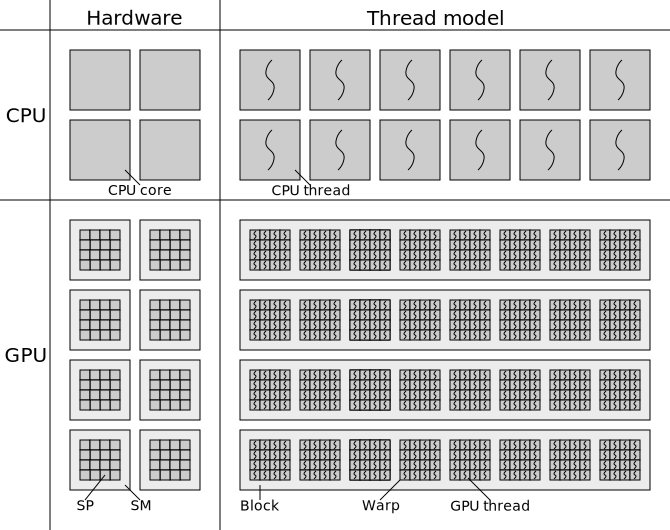
\includegraphics[width=\linewidth]{gpu-vs-cpu.png}
	\caption{
		Graphical representation of the analogy between hardware and thread model on CPUs and GPUs.
		Each CPU core can work on one thread at a time, so threads are managed individually.
		Each SM can work on multiple threads at once so threads are managed as warps.
		Warps are in turn grouped together as blocks.
	}
	\label{gpu-vs-cpu}
\end{figure*}

The difference in architectures between CPUs and GPUs is reflected in how they organize threads (compare figure \ref{gpu-vs-cpu}).
A CPU has one or more cores that execute threads one at a time, so threads are being managed as single threads.
A GPU has many so-called \textit{streaming multiprocessors} (SM) that in turn consist of many \textit{streaming processors} (SP).
The SPs on an SM synchronously run threads with the same instructions that are combined to a so-called \textit{warp}.
Each SM manages multiple warps which are in turn combined to \textit{blocks};
these are the units that are being assigned to an SM.

Each warp in a block executes the same code.
When a block is assigned to SM it begins to execute one of the warps in the block until no more work can be done on the warp
(e.g. because the warp needs to fetch data from memory).
The SM then performs a \textit{context switch} to another warp in the same block and continues to do work.
Ideally, the reason why one particular warp cannot do work will be resolved while the SM works on the other warps
(for example because the data arrives from memory).
In this case no time at all was spent waiting from the perspective of a single warp.
This practice is called \textit{latency hiding}.

It is important to note that unlike CPU cores, SPs do not have dedicated registers.
Instead they share the registers of the SM and these registers are \textbf{not} flushed upon a context switch.
This means that context switches between warps can be performed very quickly.
However, it also means that registers are shared between warps, reducing the number of available registers per warp.
Large warps can result in the eviction of registers used by other warps to memory, inducing latency on a context switch.

Due to the differences in their architectures multi-threading on a GPU
is utilized very differently when compared to multi-threading on a CPU.
On a CPU threads are very expensive and the overhead cost associated with
creating a large number of threads can outweigh the benefits gained from parallelism;
a common strategy for maximizing performance on a CPU is to create as many threads as there are logical CPU cores.
On a GPU however threads are extremely lightweight by comparison;
a common strategy for maximizing performance on a GPU is to create
many times more small threads than there are SPs to ensure that the GPU never runs out of work to do.

The difference in thread management described above reflects the difference in design goals between CPUs and GPUs.
CPUs are optimized for the execution of code that frequently branches (in terms of conditional statements or loops).
They have a large number of registers and large amounts of cache per CPU core to reduce the latency induced by memory accesses.
GPUs on the other hand are optimized for computational bandwidth.
They have a much larger number of comparatively slower SPs that are designed to run code with limited branching.
Because SPs have access to fewer registers and less cache than CPU cores GPUs are also more suited for code that
accesses data only once rather than many times.

\section{Programming GPUs}
\label{sec:programming}
CUDA\cite{cuda} and OpenCL\cite{opencl}, two of the most widely used GPU computing frameworks function very similarly from the perspective of a programmer:
they both extend the C programming language\cite{c} with some functionality to run code on GPUs.
Because they are based on C these frameworks feature manual memory management but with a twist:
since discrete GPUs come with their own memory it's necessary to manually move data between
GPU and system memory with a special function (see figure \ref{memory-transfer}).
\begin{figure*}
	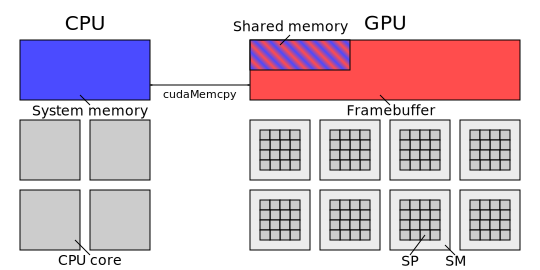
\includegraphics[width=\linewidth]{memory-transfer.png}
	\caption{
		Graphical representation of the transfer of data between memory accessible by the CPU (system memory)
		and the GPU (frame buffer).
		The data is transferred with a special function
		(CUDA's cudaMemcpy in this case, other frameworks have equivalent functions).
	}
	\label{memory-transfer}
\end{figure*}

The parallelism of a GPU can be exploited by writing so-called \textit{kernels}, functions to be executed on the GPU.
When these kernels are launched the GPU creates and runs a large number of threads on the GPU as parameterized by the program.
In accordance with the single instruction, multiple thread execution model these threads all run the same kernel code in sync.
To coordinate these threads they each receive one or more indices that can for example
be used to determine which portion of the input data a thread should be working on.

Compared to low-level GPU programming frameworks like CUDA and OpenCL there are also high-level frameworks like
Tensorflow\cite{tensorflow} which are capable of utilizing GPUs.
Instead of executing explicitly supplied GPU kernels these high-level frameworks automatically generate these kernels from
operations performed on vectorized data structures.
This allows for a separation of the calculation logic and the (hardware-specific) implementation of a calculation.
As a consequence the same code can be executed on both CPUs and GPUs.
As long as the calculation can be expressed as a combination of operations that can be efficiently parallelized
(see section \ref{sec:ppp}) the performance will scale well.
\section{Parallel Programming Patterns}
\label{sec:ppp}
This section describes a few fundamental patterns that are commonly used to create parallel programs.
They can be efficiently parallelized on both CPUs and GPUs and are provided as fundamental operations in frameworks like Tensorflow.
Note that the patterns described here are not exclusive to (GPU-accelerated) parallel programming.
The \textit{map}, \textit{filter}, and \textit{fold} (generalization of \textit{reduce}) patterns for instance are essential for functional programming.

For the following considerations let us assume that we have a GPU with $M$ streaming processors.
Let $x$ be an array with length $N$ (measured by number of elements, not bytes).
The elements of this array $x_n$ have data type $t_x$.

The phrase ''\textit{separating x into segments}'' is to be interpreted as separating $x$ into $M$ segments of equal size;
we can assume without loss of generality that $N$ is divisible by $M$.
A pattern is considered \textit{embarrassingly parallel} if the speedup of the pattern as a whole
is approximately proportional to the number of SPs used.
\subsection{Map}
\label{map}
The \textit{map} pattern works by applying a function $f: t_x \rightarrow t_y$
to all values of $x$ to produce another array $y$ with the same length:
\begin{equation}
	y_n = f(x_n), \quad 0 \le n < N.
\end{equation}
Notably the values of $y$ can be calculated independently from one another;
if the execution of $f$ takes a constant amount of time the task of mapping $x$ to $y$ can be parallelized very efficiently.
First $x$ is divided into segments and each segment is assigned to a different SP.
Then each SP simply applies $f$ to the values in its segment in parallel.
An example is shown in figure \ref{fig:map}.
\begin{figure*}
	\centering
	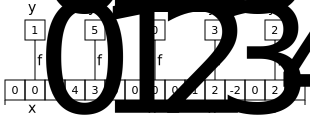
\includegraphics[width=\textwidth]{pattern-map.png}
	\caption{
		Visualization of the map pattern.
		3-vectors are mapped to their lengths.
		Because the two data types have different sizes the operation is not performed in-place.
	}
	\label{fig:map}
\end{figure*}
If $t_x$ and $t_y$ have the same size map can be performed in-place, requiring only $O(M)$ extra memory.
If $x$ needs to be re-used or if $t_x$ and $t_y$ have different sizes a new array needs to be allocated for $y$.
Under the assumption that $f$ takes a constant amount of time to compute map is embarrassingly parallel.
\subsection{Reduce}
\label{reduce}
The \textit{reduce} pattern condenses all values of $x$ into a single value $y$.
In order for this pattern to work $y$ must have the same data type as $x_i$ and
there must be an associative operator $\oplus: (t_x, t_x) \rightarrow t_x$ that carries out the reduction.
A simple way to implement the reduce pattern is to again divide $x$ into segments and assign each segment to a different SP.
Then each segment is reduced with $\oplus$ to a single value $y_n$.
The values $y_n$ can then in turn be iteratively reduced:
first $\frac{N}{2}$ SPs reduce the $y_n$ to just $\frac{N}{2}$ values while $\frac{N}{2}$ SPs are idling,
then $\frac{N}{4}$ SPs reduce the $\frac{N}{2}$ from the previous iteration to $\frac{N}{4}$ new values while $\frac{3N}{4}$ SPs are idling,
and so on until the $y_n$ have been reduced to a single value.
An example is shown in figure \ref{fig:reduce}.
\begin{figure*}
	\centering
	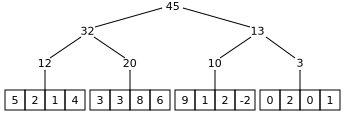
\includegraphics[width=\textwidth]{pattern-reduce.png}
	\caption{
		Visualization of the reduce pattern.
		Integers are summed up to a single value.
		In this example four streaming processors/CPU cores are used.
	}
	\label{fig:reduce}
\end{figure*}

The implementation described above is embarrassingly parallel if $N >> M$.
In this case the work of reducing the individual segments into $y_n$ is dominant
and the SPs will only spend a small amount of time idling at the end.
The described implementation would also only require $O(M)$ extra memory and have a runtime of $O(N)$.

As an example, let us consider calculating the sum of an array of integers.
With the reduce pattern each SP would sum up part of the array to create partial sums.
The partial sums are then iteratively added up to the total sum of the array.

In regards to sums there is an important caveat though:
most operations on floating point numbers, particularly additions, are \textbf{not} associative.
Because floating point numbers only have a limited precision their operations are subject to rounding errors.
As such, applying the parallel reduce pattern to an array of floating point numbers will usually yield a slightly different result
compared to a sequential execution.
The techniques for minimizing the floating point error are the same for sequential and parallel execution though,
and they are as such beyond the scope of this document.
\subsection{Filter}
The \textit{filter} pattern is - as the name implies - used to filter an array based on some criterion:
elements that fulfill the criterion are kept while elements that don't are discarded.
This can be achieved by defining a function $f: t_x \rightarrow \textbf{bool}$ and keeping only those elements $x_i$
where $f(x_i)$ is evaluated to \textit{true}.
As with map the filter pattern for a single element $x_n$ can be evaluated independently from all other elements.
As such, the same simple strategy of separating $x$ into segments and working on each segment in parallel can be used.
However, because the array produced by the filter pattern is of a different size
compared to the input array the filter pattern cannot be performed in-place.
The elements filtered by each SP need to be copied to a new array and possibly copied again at the end to form a contiguous array.
An example is shown in figure \ref{fig:filter}.
\begin{figure*}
	\centering
	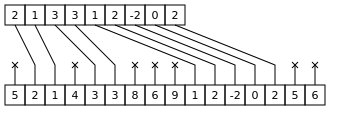
\includegraphics[width=\textwidth]{pattern-filter.png}
	\caption{
		Visualization of the filter pattern.
		Only integers smaller than 4 are accepted.
		The operation is not in-place.
	}
	\label{fig:filter}
\end{figure*}

The implementation described above is embarrassingly parallel if $N >> M$
since in this case the time needed for filtering the segments is dominant.
Due to having to create a new array the described implementation is $O(N)$ both in terms of extra memory and runtime.

\section{Simple Benchmark}
To better illustrate the benefits of GPUs we performed a few simple benchmarks:
we timed the MC calculation of $\pi$ on a GPU using the Tensorflow (v2.5.0-2) package and compared it
to an equivalent implementation using the NumPy (v1.20.3-1) package.
All benchmarks were performed on a Linux platform using a Ryzen 3700X CPU and an NVIDIA GTX 1070 GPU.
The CPU and GPU are roughly equal in terms of price and release date.
\subsection{Hit-And-Miss MC}
The calculation of $\pi$ using hit-and-miss MC can be implemented with the following Python code:
\begin{lstlisting}
@tf.function
def mc_tf(sample_size):
    rand_xy = tf.random.uniform(
	(sample_size, 2))

    # Map:
    in_circle = tf.square(rand_xy[:, 0]) \
	+ tf.square(rand_xy[:, 1]) < 1.0

    # Reduce:
    mc_estimate = tf.math.count_nonzero(
	in_circle) / sample_size

    return 4 * mc_estimate
\end{lstlisting}
Notably the entire calculation can be expressed as a combination of map and reduce operations,
implying that it can be efficiently parallelized on GPUs.
\begin{figure*}
	\centering
	\includegraphics[width=\linewidth]{pi_hit_and_miss_benchmark.png}
	\caption{
		Benchmark of hit-and-miss MC.
		Runtime with NumPy is proportional to sample size.
		Runtime with Tensorflow is constant for $N \le 10^7$.
		Runtime with Tensorflow is proportional to sample size for $N \ge 10^9$
		(assuming Tensorflow is already initialized).
	}
	\label{fig:pi_hit_and_miss_benchmark}
\end{figure*}
Figure \ref{fig:pi_hit_and_miss_benchmark} shows the result of the benchmark.
The runtime with NumPy (single CPU core) is proportional to sample size, indicating negligible overhead.
The runtime with Tensorflow (GPU) is flat for small sample sizes and proportional to sample size for large sample sizes,
indicating significant overhead.
For small sample sizes NumPy is much faster than Tensorflow, for large sample sizes Tensorflow is much faster than NumPy.

A large part of the GPU overhead is due to the initialization of the Tensorflow library which is several gigabytes in size.
However, some overhead still remains when this is accounted for.
The reason for this overhead is the memory management described in section \ref{sec:programming}.
Compared to computation memory accesses are very slow.
Memory transfers between system memory and GPU memory are even slower.
To execute the above code on a GPU the generated kernel needs to first be transferred to GPU memory.
After executing code the result needs to be transferred back to system memory.
For small sample sizes the runtime is entirely dominated by the memory transfers,
resulting in a runtime that is essentially constant.
For large sample sizes the time needed for memory transfers becomes negligible,
resulting in a runtime that is proportional to sample size.
\subsection{Crude MC}
The calculation of $\pi$ using crude MC can be implemented with the following Python code:
\begin{lstlisting}
@tf.function
def mc_tf(sample_size):
    rand_x = tf.random.uniform(
	(sample_size,))

    # Map:
    function_values = 1.0 - tf.math.sqrt(
	1.0 - tf.math.square(rand_x))

    # Reduce:
    mc_estimate = tf.reduce_mean(
	function_values)

    return 4 * mc_estimate
\end{lstlisting}
Again, the entire calculation can be expressed as a combination of map and reduce operations.
\begin{figure*}
	\includegraphics[width=\linewidth]{pi_crude_benchmark.png}
	\caption{
		Benchmark of crude MC.
		Runtime with NumPy is proportional to sample size.
		Runtime with Tensorflow (GPU) is constant for $N <= 10^7$.
		Runtime with Tensorflow (CPU and GPU) is proportional to sample size for $N >= 10^9$
		(assuming Tensorflow is already initialized).
	}
	\label{fig:pi_crude_benchmark}
\end{figure*}
Figure \ref{fig:pi_crude_benchmark} shows the result of the benchmark.
The results for NumPy and Tensorflow (GPU) are essentially the same as for the hit-and-miss implementation.
Additionally to Tensorflow (GPU) we also benchmarked Tensorflow (CPU) to investigate the runtime
of a multithreaded CPU implementation.
Just like with Tensorflow (GPU) there is significant overhead that becomes negligible for large sample sizes.
The overhead is due to the cost associated with thread creation.
At least in this benchmark Tensorflow (GPU) was always faster than Tensorflow (CPU), particularly for large sample sizes.

\section*{Conclusion}
\addcontentsline{toc}{section}{Conclusion}
In this paper we introduced the techniques hit-and-miss MC and crude MC.
We showed how crude MC can be improved with importance sampling and how this process can be automated with the VEGAS algorithm.

We gave a breakdown of the architecture of (modern) GPUs and how this corresponds to their thread model
and the frameworks used to program them.

We illustrated the programming patterns map, reduce, and filter, and how they can be efficiently parallelized using an SIMT architecture.

Finally, we performed a simple benchmark of MC calculation and found that GPUs outperformed CPUs for large sample sizes
but introduced significant latency due to memory transfers.


%------------------------------------------------

\phantomsection
\section*{Acknowledgments} % The \section*{} command stops section numbering

\addcontentsline{toc}{section}{Acknowledgments} % Adds this section to the table of contents

Thank you, Ulrich Husemann for providing guidance when composing this paper and the corresponding presentation.

%----------------------------------------------------------------------------------------
%	REFERENCE LIST
%----------------------------------------------------------------------------------------

\phantomsection
\bibliographystyle{unsrt}
\bibliography{main.bib}

%----------------------------------------------------------------------------------------

\end{document}
